\section{Obtaining \texorpdfstring{$\phi$}{the potential}}
%
We observe the dependency of $\phi$ in \cref{eq:celma_dens,eq:celma_mom_dens,eq:celma_j_par,eq:celma_vortD_evolution}, but that $\phi$ is not described by a initial boundary value problem equation.
Instead, we must find alternative ways of extracting $\phi$.
We will in the following discuss two ways of doing so.
% TODO: Delete me if not in thesis
%       extra/constraint can be inserted here

\subsection{As a matrix inversion problem}
%
The problem of obtaining $\phi$ can be posed as a matrix problem $A\ve{x}=\ve{b}$, where $\ve{x}$ is an array of all the spatial values of $\phi$ ordered in some way, and $\ve{b}$ is an array of all the spatial values of $\Omega^D$ ordered in the same way.
Since we are working in an orthogonal coordinate system, we have that $\Om^D = \div\L(n\frac{\grad_\perp\phi}{B}\R) = \grad_\perp\cdot\L(n\frac{\grad_\perp\phi}{B}\R)$, as no basis vector parallel to the magnetic field can be obtained from taking the derivative of the vector $n\frac{\grad_\perp\phi}{B}$, which has only perpendicular components.
Thus, in our case, we can solve the $A\ve{x}=\ve{b}$ system for each plane perpendicular to the magnetic field.
That is, our matrix $A$ would be a $n_x \times n_y$ matrix, where $n_x$ and $n_y$ is the number of points for the two perpendicular directions
%
\footnote{
Note that in the BOUT++ implementation, $y$ is chosen as the direction parallel to the magnetic field.
This is due to historical reasons.
$n_y$ would be named $n_z$ in BOUT++ convention.
In order not to confuse readers unfamiliar with BOUT++, $z$ is chosen as the coordinate along the magnetic field unless other is specified.
}%
%
.
We note that if $\div\L(n\frac{\grad_\perp\phi}{B}\R)$ were not purely perpendicular, we would have to solve $A\ve{x}=\ve{b}$ for the whole domain.
In other words, the size of matrix $A$ would be $n_x \times n_y \times n_z$, and would be considerably harder to solve numerically.

As noted in \cite{Wiesenberger2014Phd} (in the case where $P=1$, that is, in the finite difference case), the discretization of the elliptic equation $\div\L(n\frac{\grad_\perp\phi}{B}\R)=\Om^D$ can be formulated in a symmetric manner, when special care is taken at the boundary.

Solving for the ghost-point, meaning that the ghost-point would be one of the unknown in $A\ve{x}=\ve{b}$, would break the symmetry.
Instead, one must reformulate the boundary condition in a way such that it becomes an equation for the ghost point.
The equation of the ghost point can then be substituted into the equations for the first/last inner point (the point just before the boundary) and thus effectively eliminating the ghost point from the set of equations.

To exemplify, consider a second order Dirichlet boundary condition with the boundary half between grid points for the equation $\partial_x^2 f = b$, where $f_{-1}$ denotes the value at the ghost point, $f_{\text{BC}}$ denotes the value at the boundary and $f_{1}$ denotes the value at the first inner ghost point.
The boundary condition can now be written $\frac{f_{-1}+f_{1}}{2}=f_{\text{BC}}$, and the equation for the first inner point could be written $\frac{f_{-1}+2f{1}+f_{2}}{(\Delta x)^2}=b_1$.
This would lead to the equation system
%
\begin{align*}
    A\cdot\ve{f}=&\ve{b}\\
    %
    \frac{1}{(\Delta x)^2}
    \begin{bmatrix}
        (\Delta x)^2\frac{1}{2} & (\Delta x)^2\frac{1}{2} & 0 & 0 & \ldots\\
        1                       & 2                       & 1 & 0 & \ldots\\
        0                       & 1                       & 2 & 1 & \ldots\\
        \vdots                  & \vdots              &\vdots&\vdots&\ddots\\
    \end{bmatrix}
    \cdot
    \begin{bmatrix}
        f_{-1}\\
        f_{1}\\
        f_{2}\\
        f_{3}\\
        \vdots
    \end{bmatrix}
    =&
    \begin{bmatrix}
        f_{\text{BC}}\\
        b_{1}\\
        b_{2}\\
        b_{3}\\
        \vdots
    \end{bmatrix}
\end{align*}
%
which is clearly non-symmetric.

The symmetric way to implement this would be to write $f_{-1}=2f_{\text{BC}}-f_{1}$ for the boundary condition, and substitute this into the 2nd order finite difference equation for the first inner ghost point.
This gives
%
\begin{align*}
    \frac{f_{-1}+2f{1}+f_{2}}{(\Delta x)^2}&=b_1\\
    \frac{2f_{\text{BC}}-f_{1}+2f{1}+f_{2}}{(\Delta x)^2}&=b_1\\
    \frac{f{1}+f_{2}}{(\Delta x)^2}&=b_1 - \frac{2f_{\text{BC}}}{(\Delta x)^2}
\end{align*}
%
This would give
%
\begin{align*}
    A\cdot\ve{f}=&\ve{b}\\
    %
    \frac{1}{(\Delta x)^2}
    \begin{bmatrix}
        1                       & 1                       & 0 & 0 & \ldots\\
        1                       & 2                       & 1 & 0 & \ldots\\
        0                       & 1                       & 2 & 1 & \ldots\\
        \vdots                  & \vdots              &\vdots&\vdots&\ddots\\
    \end{bmatrix}
    \cdot
    \begin{bmatrix}
        f_{1}\\
        f_{2}\\
        f_{3}\\
        \vdots
    \end{bmatrix}
    =&
    \begin{bmatrix}
        b_{1} - \frac{2f_{\text{BC}}}{(\Delta x)^2}\\
        b_{2}\\
        b_{3}\\
        \vdots
    \end{bmatrix}
\end{align*}
%
which is symmetric.
Although difficult, one can show that the non-linear elliptic equation in its symmetric form can be singular positive definite and thus be solved using the conjugate gradient method.
% FIXME: Add reference

\subsection{The Naulin solver}
%
The potential can also be found in an iterative way.
The method first used by Naulin in \cite{Naulin2008} will be presented here, and will be referred to as the Naulin solver.

The method can be used as long as
%
\begin{enumerate}[noitemsep,nolistsep]
    \item $\div\L(\frac{\grad_\perp\phi}{B}\R) = \frac{\grad_\perp^2\phi}{B}$
    \item $\grad f \cdot \grad_\perp g = \grad_\perp f \cdot \grad_\perp g$
\end{enumerate}
%
Point 1. is satisfied in our system as $B$ is constant, and because derivatives of the perpendicular basis vectors does not yield parallel components in our system.
Point 2. is satisfied as the dot product of the perpendicular basis vectors and the parallel basis vector is zero.
We then get that
%
\begin{align*}
    \Om^D =& \div\L(n\frac{\grad_\perp\phi}{B}\R)\\
    %
    =& n\div\L(\frac{\grad_\perp\phi}{B}\R) +
    \frac{\grad_\perp\phi}{B}\cdot\grad n
    \\
    %
    =& n\frac{\grad_\perp^2\phi}{B} +
    \grad n\cdot\frac{\grad_\perp\phi}{B}
    \\
    %
    =& n\frac{\grad_\perp^2\phi}{B} +
    \grad_\perp n\cdot\frac{\grad_\perp\phi}{B}
    \\
    %
    \Om^D =& n\frac{\grad_\perp^2\phi}{B} +
    \grad_\perp n\cdot\frac{\grad_\perp\phi}{B}
    \\
    %
    \frac{\Om^D}{n} =& \Om +
    \frac{1}{n}\grad_\perp n\cdot\frac{\grad_\perp\phi}{B}
    \\
    %
    \Om =& \frac{\Om^D}{n} -
    \grad_\perp \ln(n) \cdot\frac{\grad_\perp\phi}{B}
\end{align*}
%
Using square bracket superscript as iteration number, the algorithm can be stated in the following way:
%
\begin{algorithm}
\begin{enumerate}[noitemsep,nolistsep]
    \item Calculate
        $ \Om^{[i]} = \frac{\Om^D}{n} -
        \grad_\perp \ln(n) \cdot\frac{\grad_\perp\phi^{[i]}}{B}
        $
    \item Invert $\grad_\perp^2 \frac{\phi^{[i+1]}}{B} = \Om^{[i]}$ by the method
        described in \cref{app:lapInv}.
    \item Calculate
        $E_{\text{abs}, L_\infty} = \max \L|\phi^{[i]} - \phi^{[i+1]}\R|$
        and
        $E_{\text{rel}, L_\infty} = \max \L|\frac{\phi^{[i]} - \phi^{[i+1]}}{\phi^{[i]}}\R|$
    \item Check whether $E_{\text{abs}, L_\infty} > \text{Tolerance}_\text{abs}$
    \begin{itemize}[noitemsep,nolistsep]
        \item If yes: Check $E_{\text{abs}, L_\infty} > \text{Tolerance}_\text{rel}$
            \begin{itemize}[noitemsep,nolistsep]
                \item If yes: Assign $\phi^{[i+1]} \to \phi^{[i]}$, increase the
                    iteration number, throw an error if the iteration number is
                    above a predefined max iteration number, if not repeat from
                    step 1.
                \item Else, if no: Stop. Function returns
            \end{itemize}
        \item Else, if no: Stop. Function returns
    \end{itemize}
\end{enumerate}
\end{algorithm}

\subsection{The inner boundary condition for \texorpdfstring{$\phi$}{the potential}}
\label{sec:innerPhiBC}
%
As mentioned in \cref{sec:BCs} there are no real inner boundary in the cylinder.
However, the inversion method described in \cref{app:lapInv} requires a boundary condition for the inner $\rho$ for each mode number.
A method to do this, first used in \cite{Naulin2008} sets the inner ghost point depending on the evenness of the mode.

If the mode is even, the mode under consideration would have the same value diametrically opposite of the innermost point.
Notice that this is true for every point sitting on the same radius.
Hence, the ghost point for the inner $\rho$ value is set to the same as the value at the innermost $\rho$.

If the mode is odd, the mode under consideration would have value of the point diametrically opposite of the innermost point, but with a changed sign.
Thus, the ghost point for the inner $\rho$ value is set to the negative of the value at the innermost $\rho$.
This is depicted in \cref{fig:BCLaplace}
%
\begin{figure}[h!]
    \centering
    \begin{subfigure}[t]{0.5\textwidth}
        \centering
        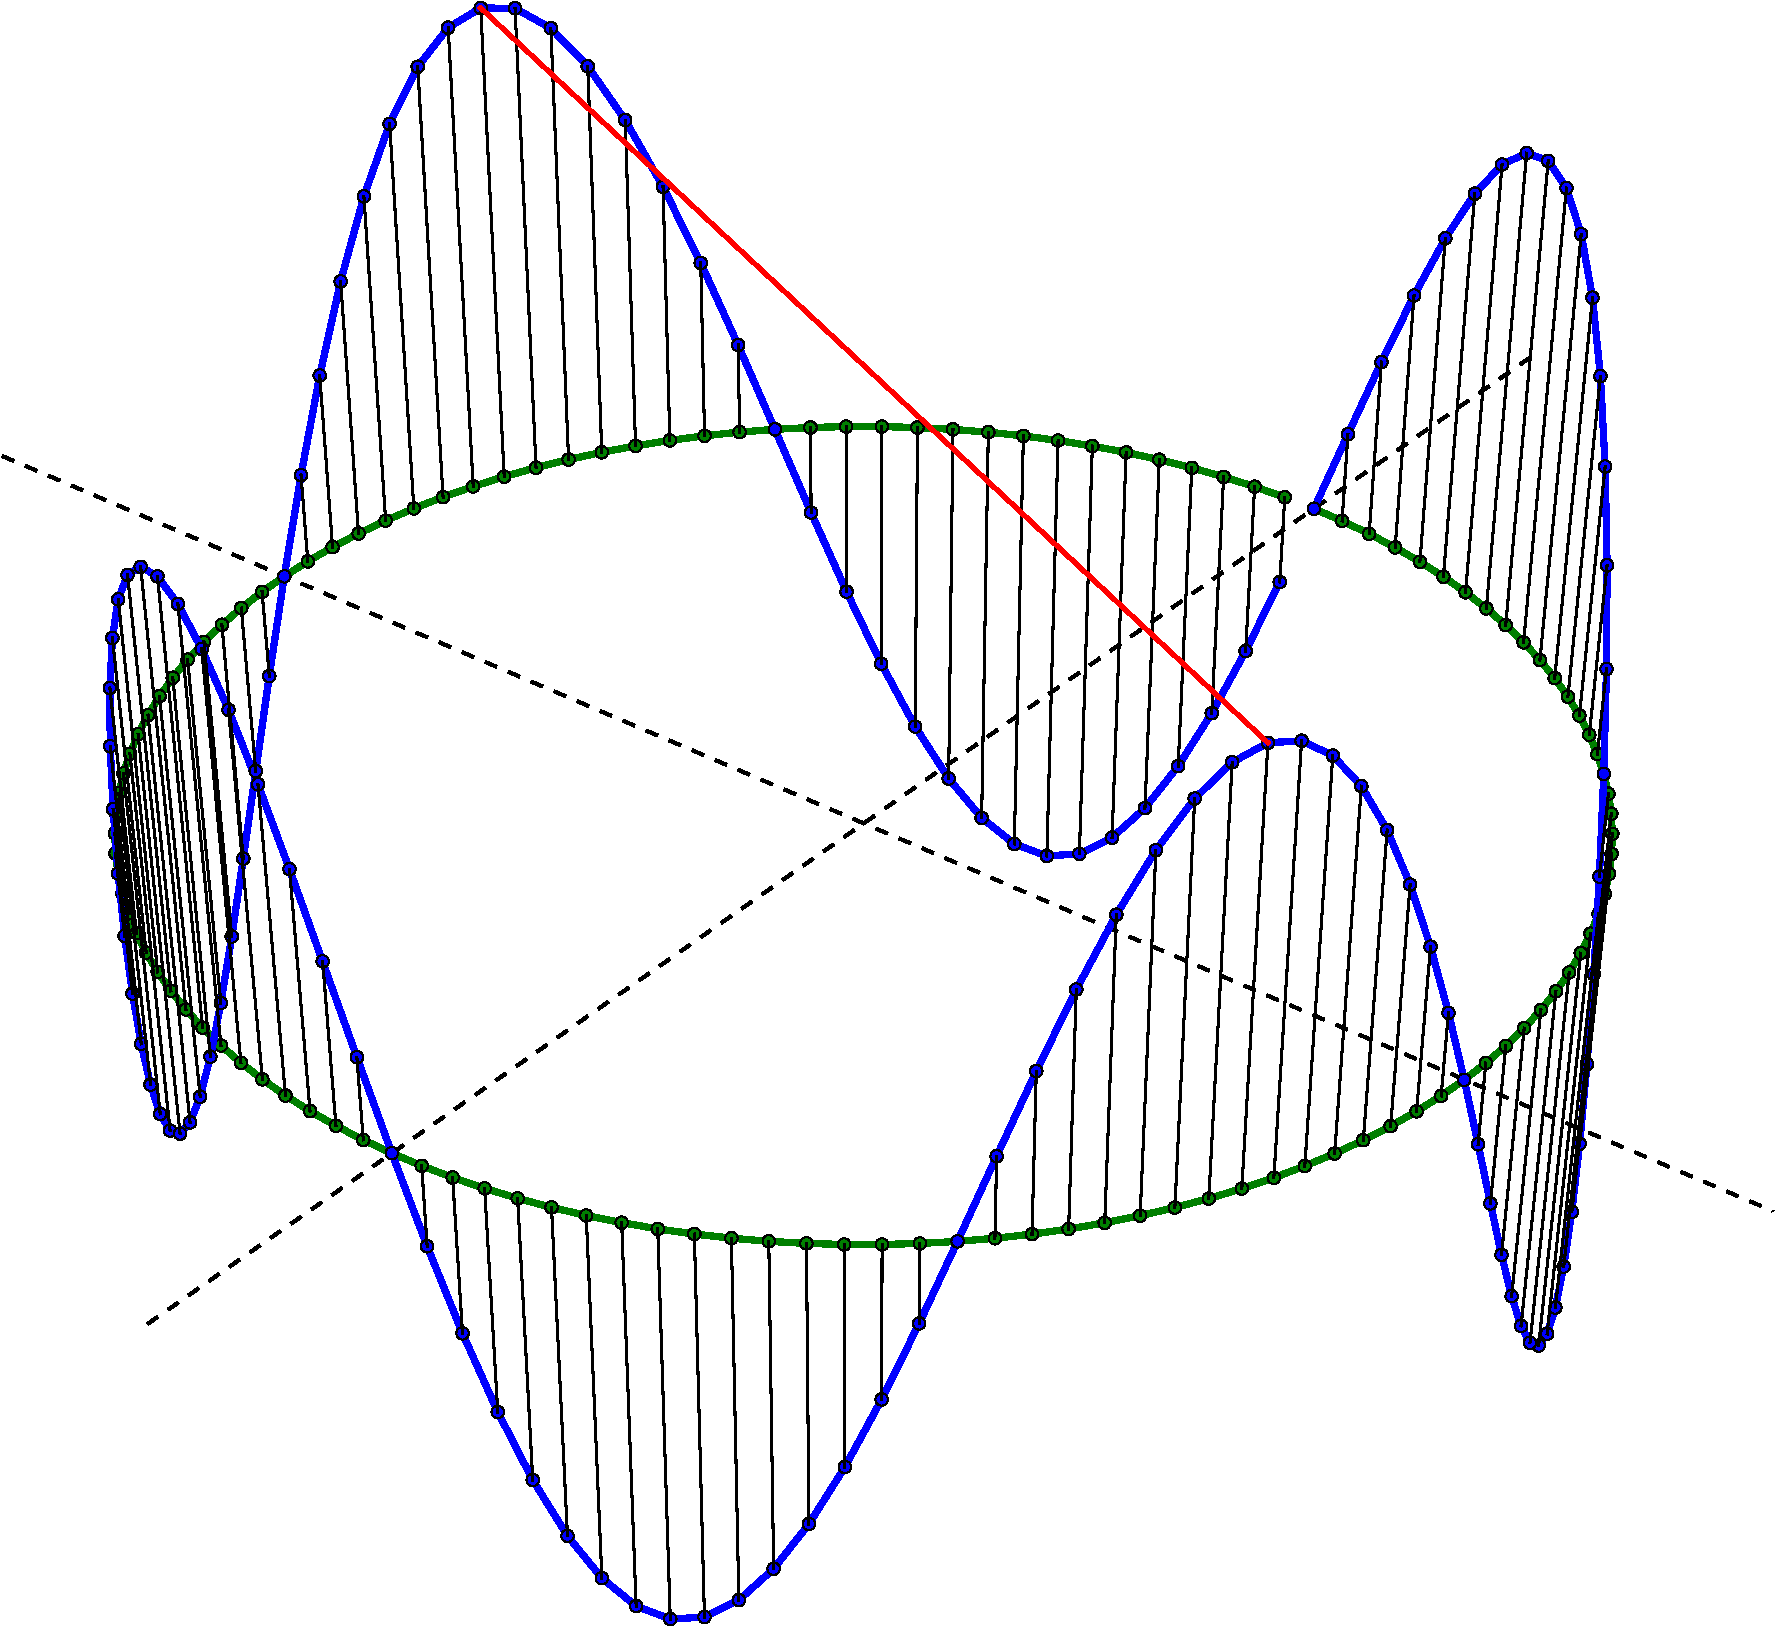
\includegraphics[width=1.0\textwidth]{fig/mode_4}
        \caption{An even mode.}
    \end{subfigure}%
    \hfill
    \begin{subfigure}[t]{0.5\textwidth}
        \centering
        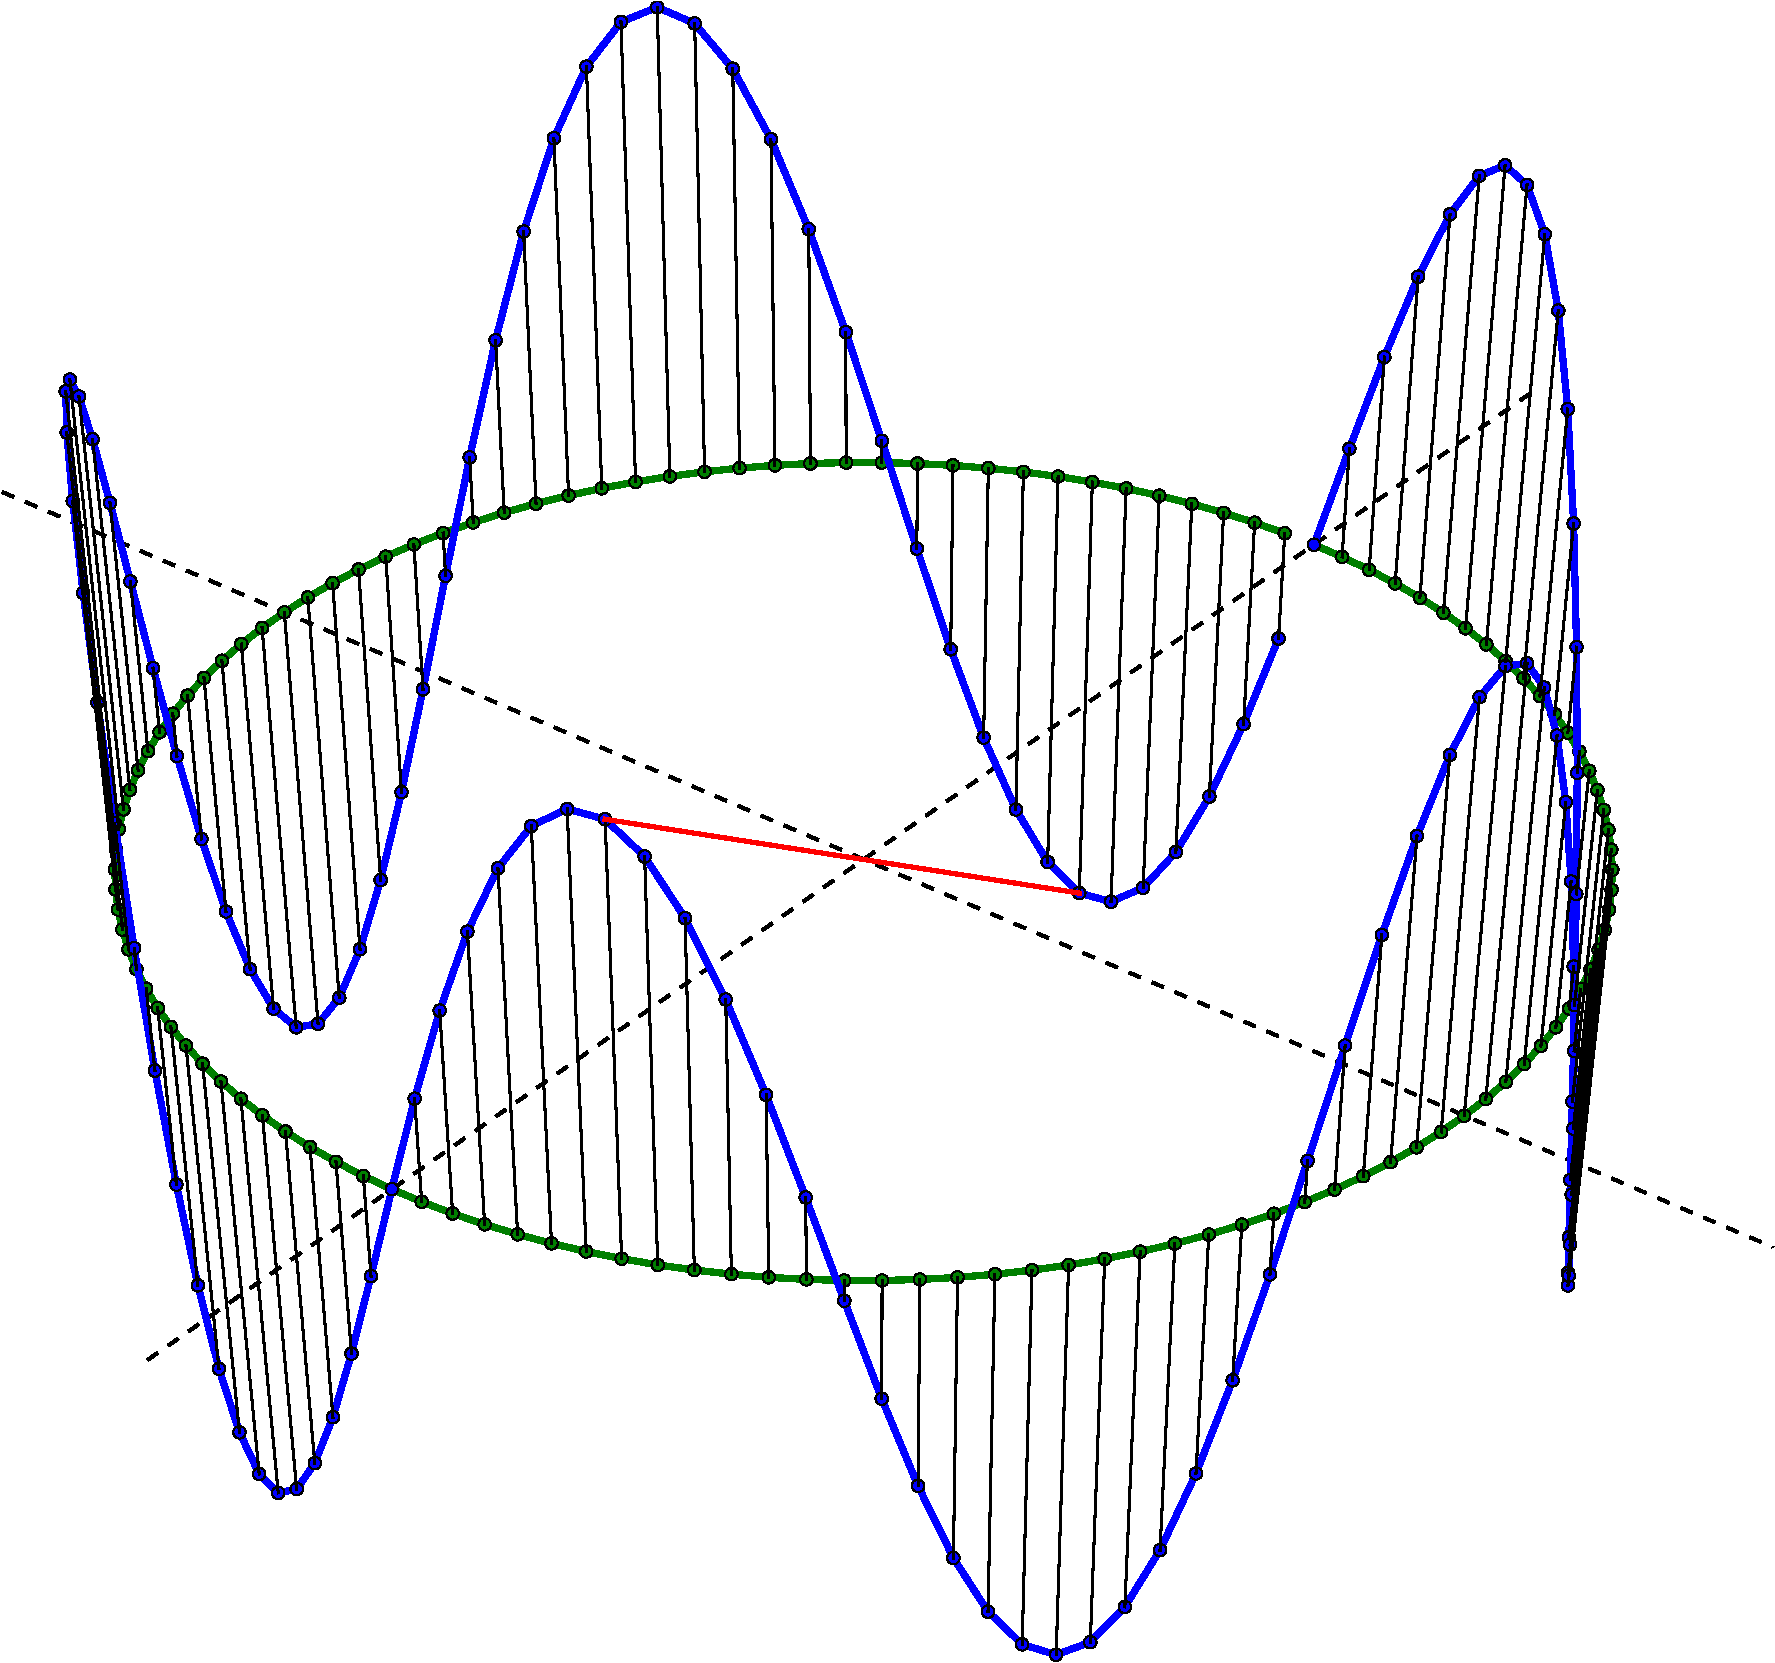
\includegraphics[width=1.0\textwidth]{fig/mode_5}
        \caption{An odd mode.}
    \end{subfigure}
        \caption{The point diametrically opposite for a mode located at radius $\rho$ has the same value as the point under consideration for an even mode, but the same value with a changed sign for even modes.
        The red soid line connects points diametrically opposite of each other.}
    \label{fig:BCLaplace}
\end{figure}
